\section{Frequency mode 21}
\label{FM21}

\subsection{Spectra}
\label{FM21:spectra}

\begin{figure}[ht]
    \centering
    \begin{subfigure}[b]{0.9545\textwidth}
        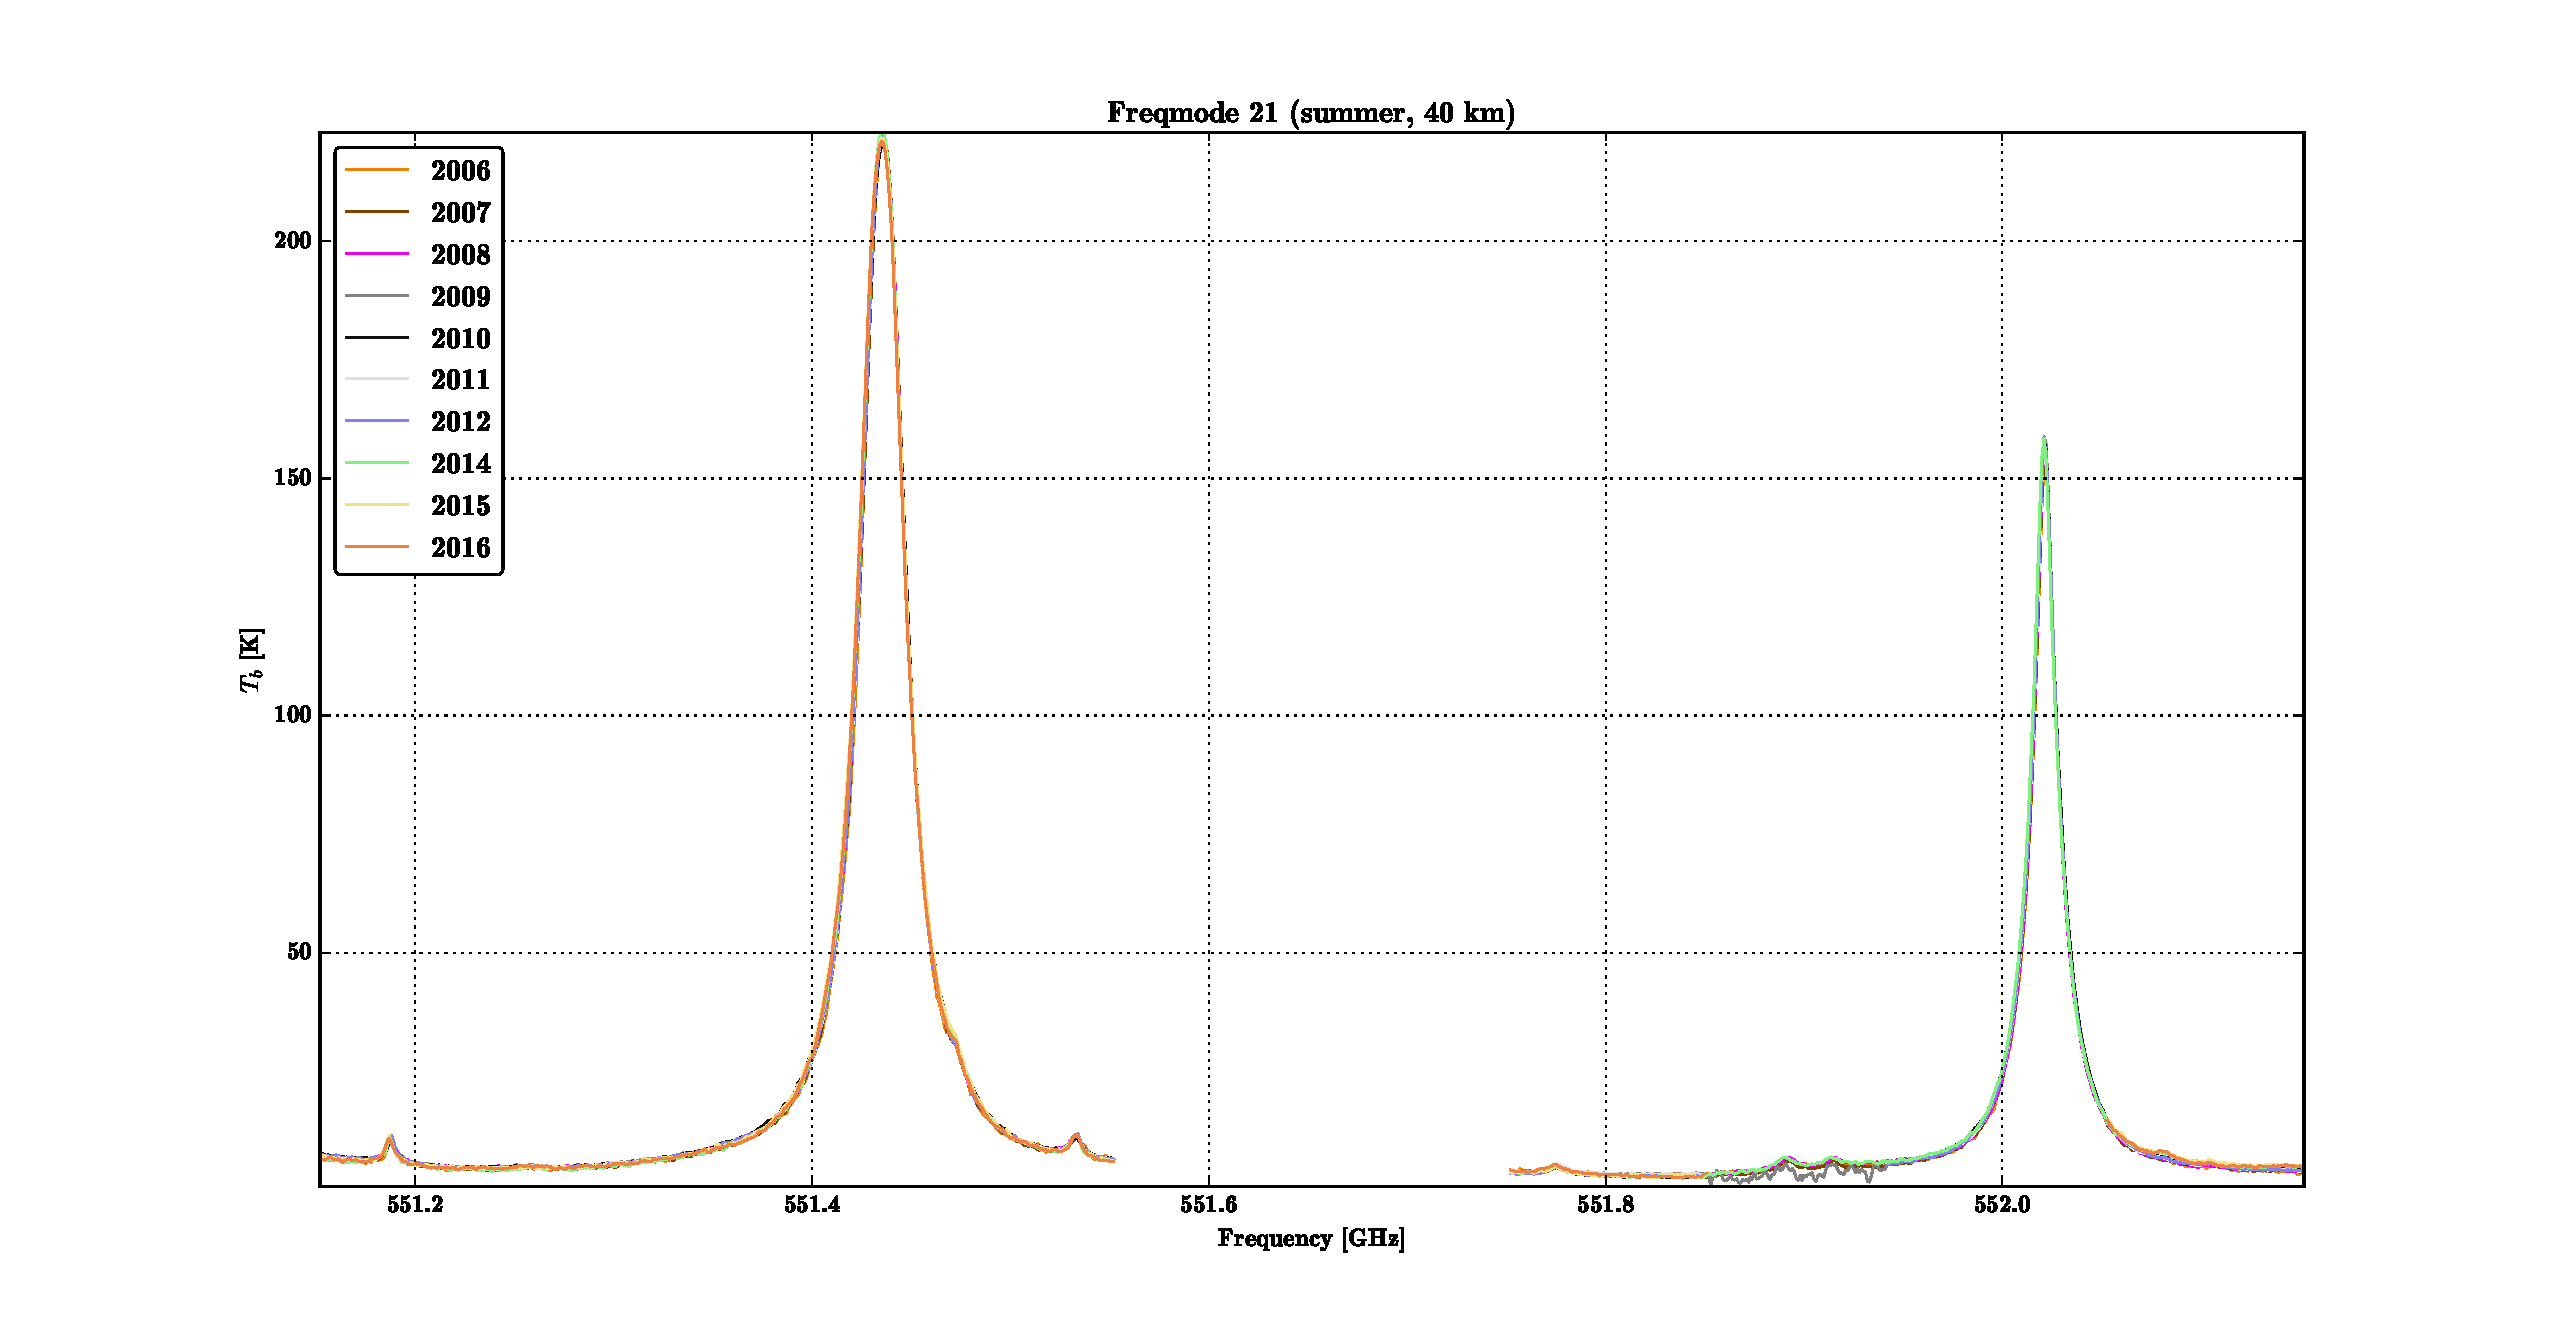
\includegraphics[width=\textwidth]{spectra/fm_21_spectra_summer}
        \caption{summer; 2014--2016 from FM~121}\label{fig:spectra:21:summer}
    \end{subfigure}
    \begin{subfigure}[b]{0.9545\textwidth}
        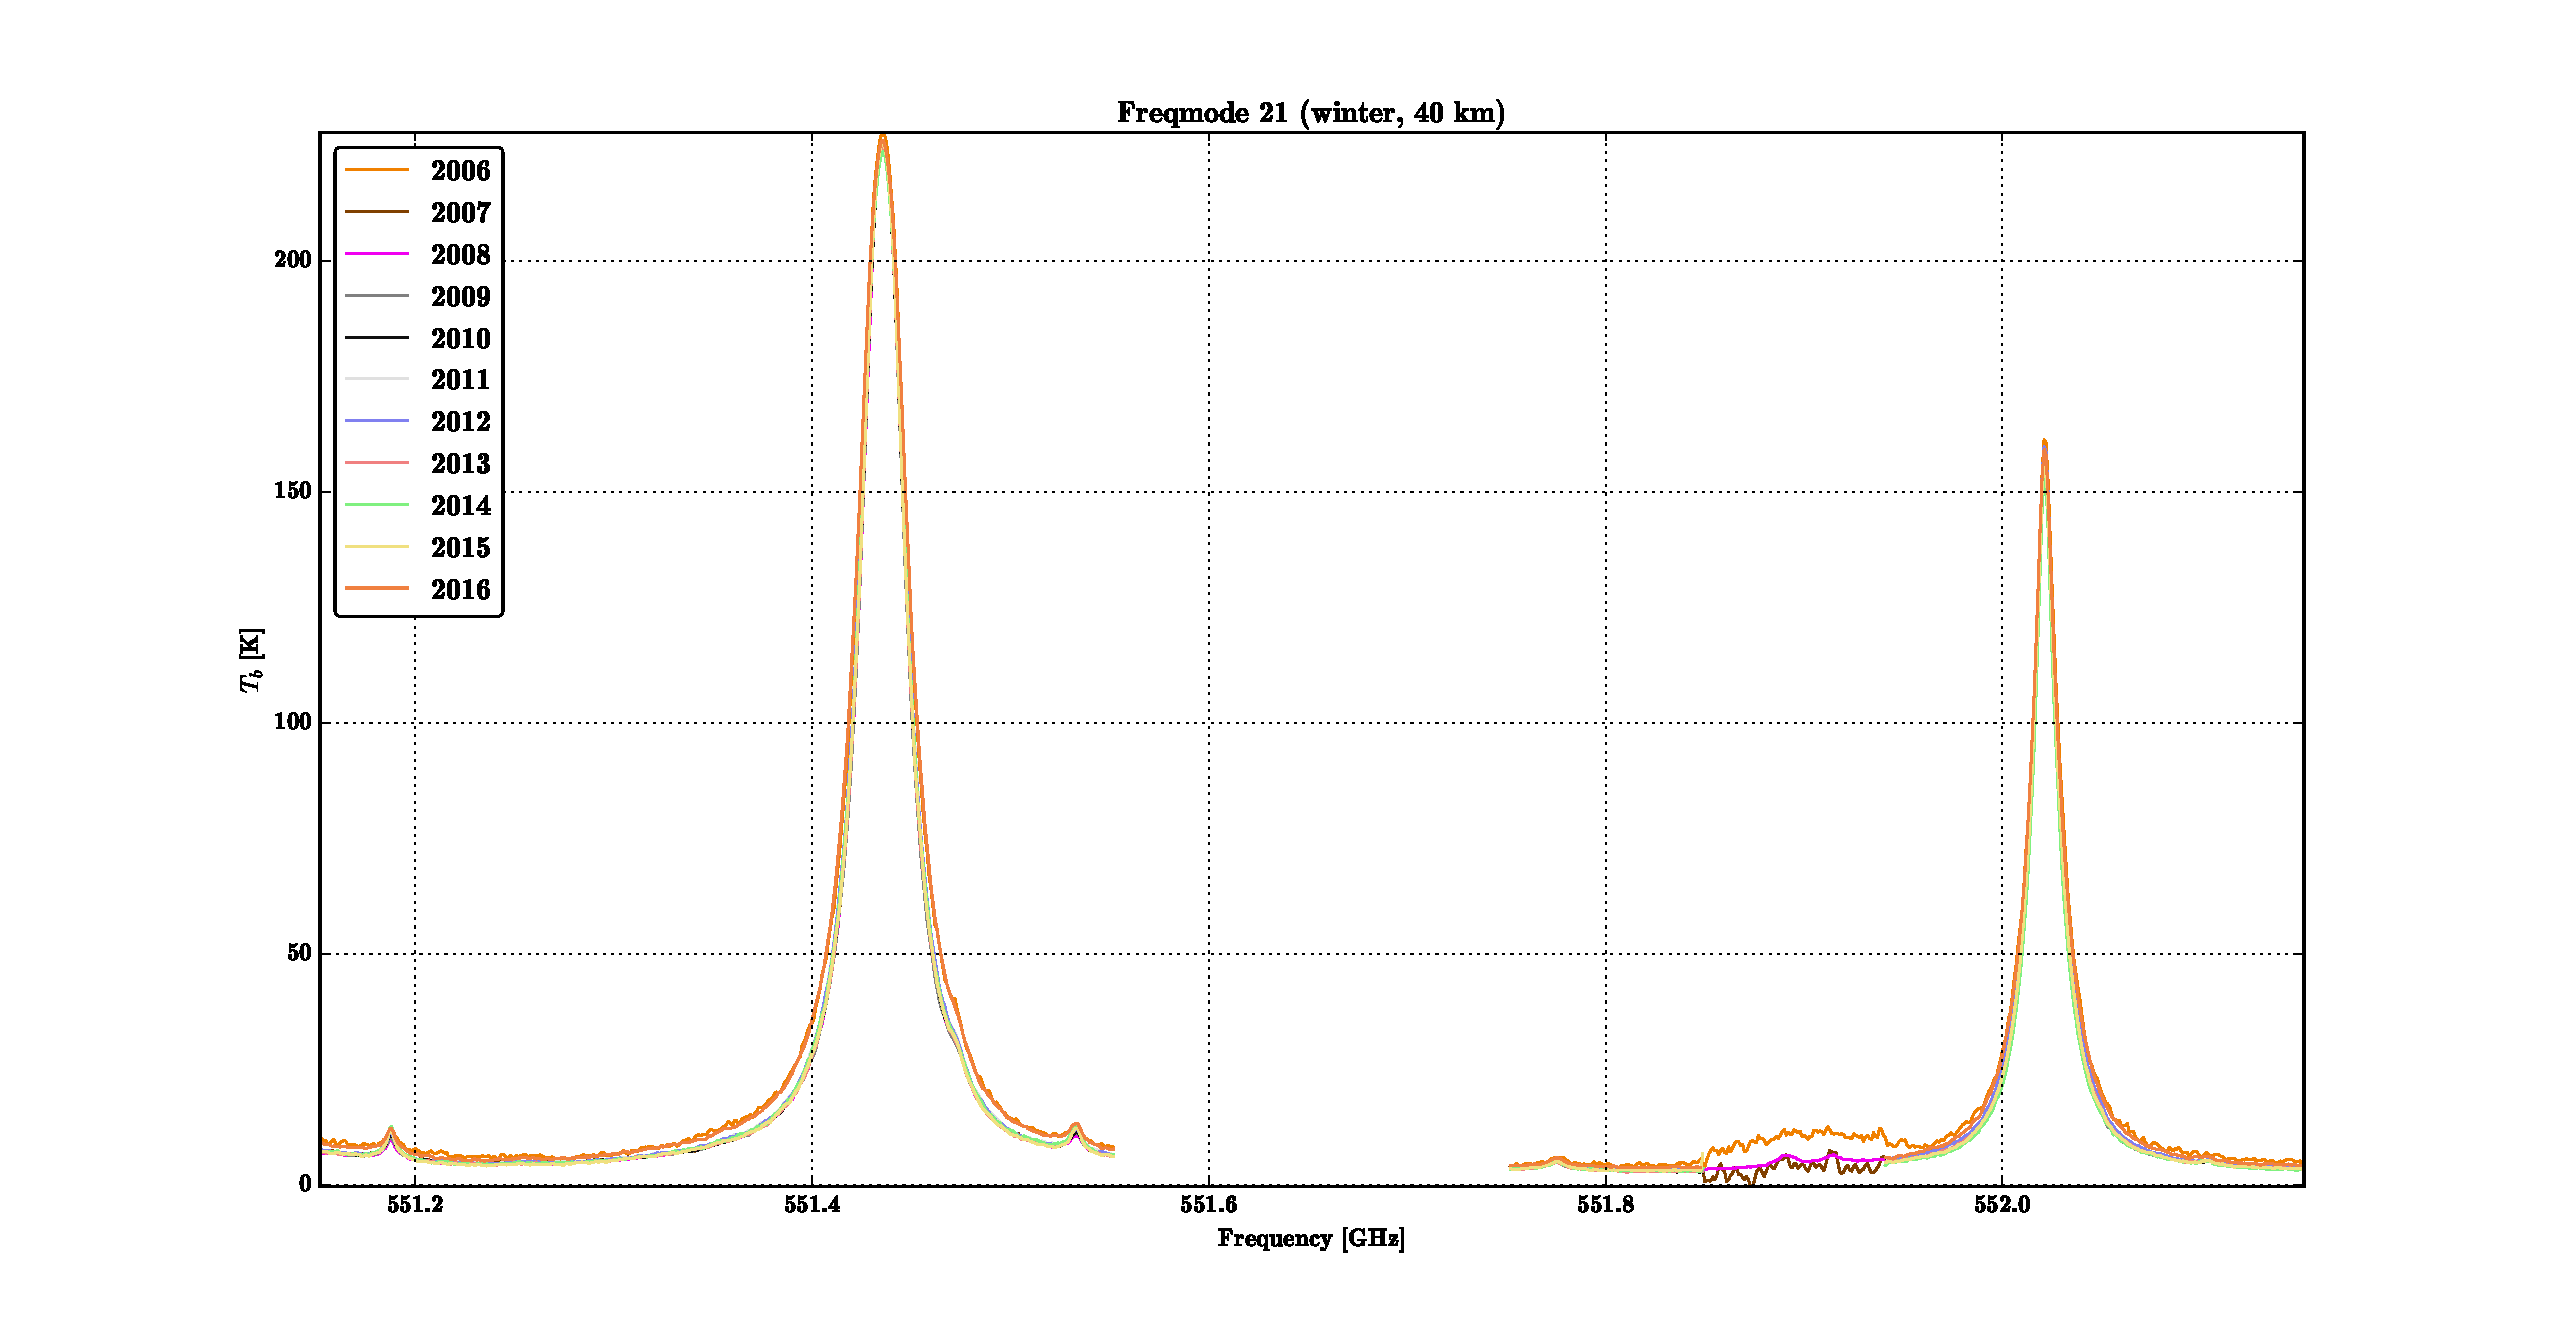
\includegraphics[width=\textwidth]{spectra/fm_21_spectra_winter}
        \caption{winter}\label{fig:spectra:21:winter}
    \end{subfigure}
    \caption{Annual median spectra for FM~21 for altitude interval 35--45~km at
        equatorial latitudes. The unhealthy sub-bands 2 and 1 are to the right
        of the gap in the middle, between~$\sim551.75$
        and~$551.95\,\mathrm{GHz}$.
        }\label{fig:spectra:21}
\end{figure}

\begin{figure}[ht]
    \centering
    \begin{subfigure}[b]{0.9545\textwidth}
        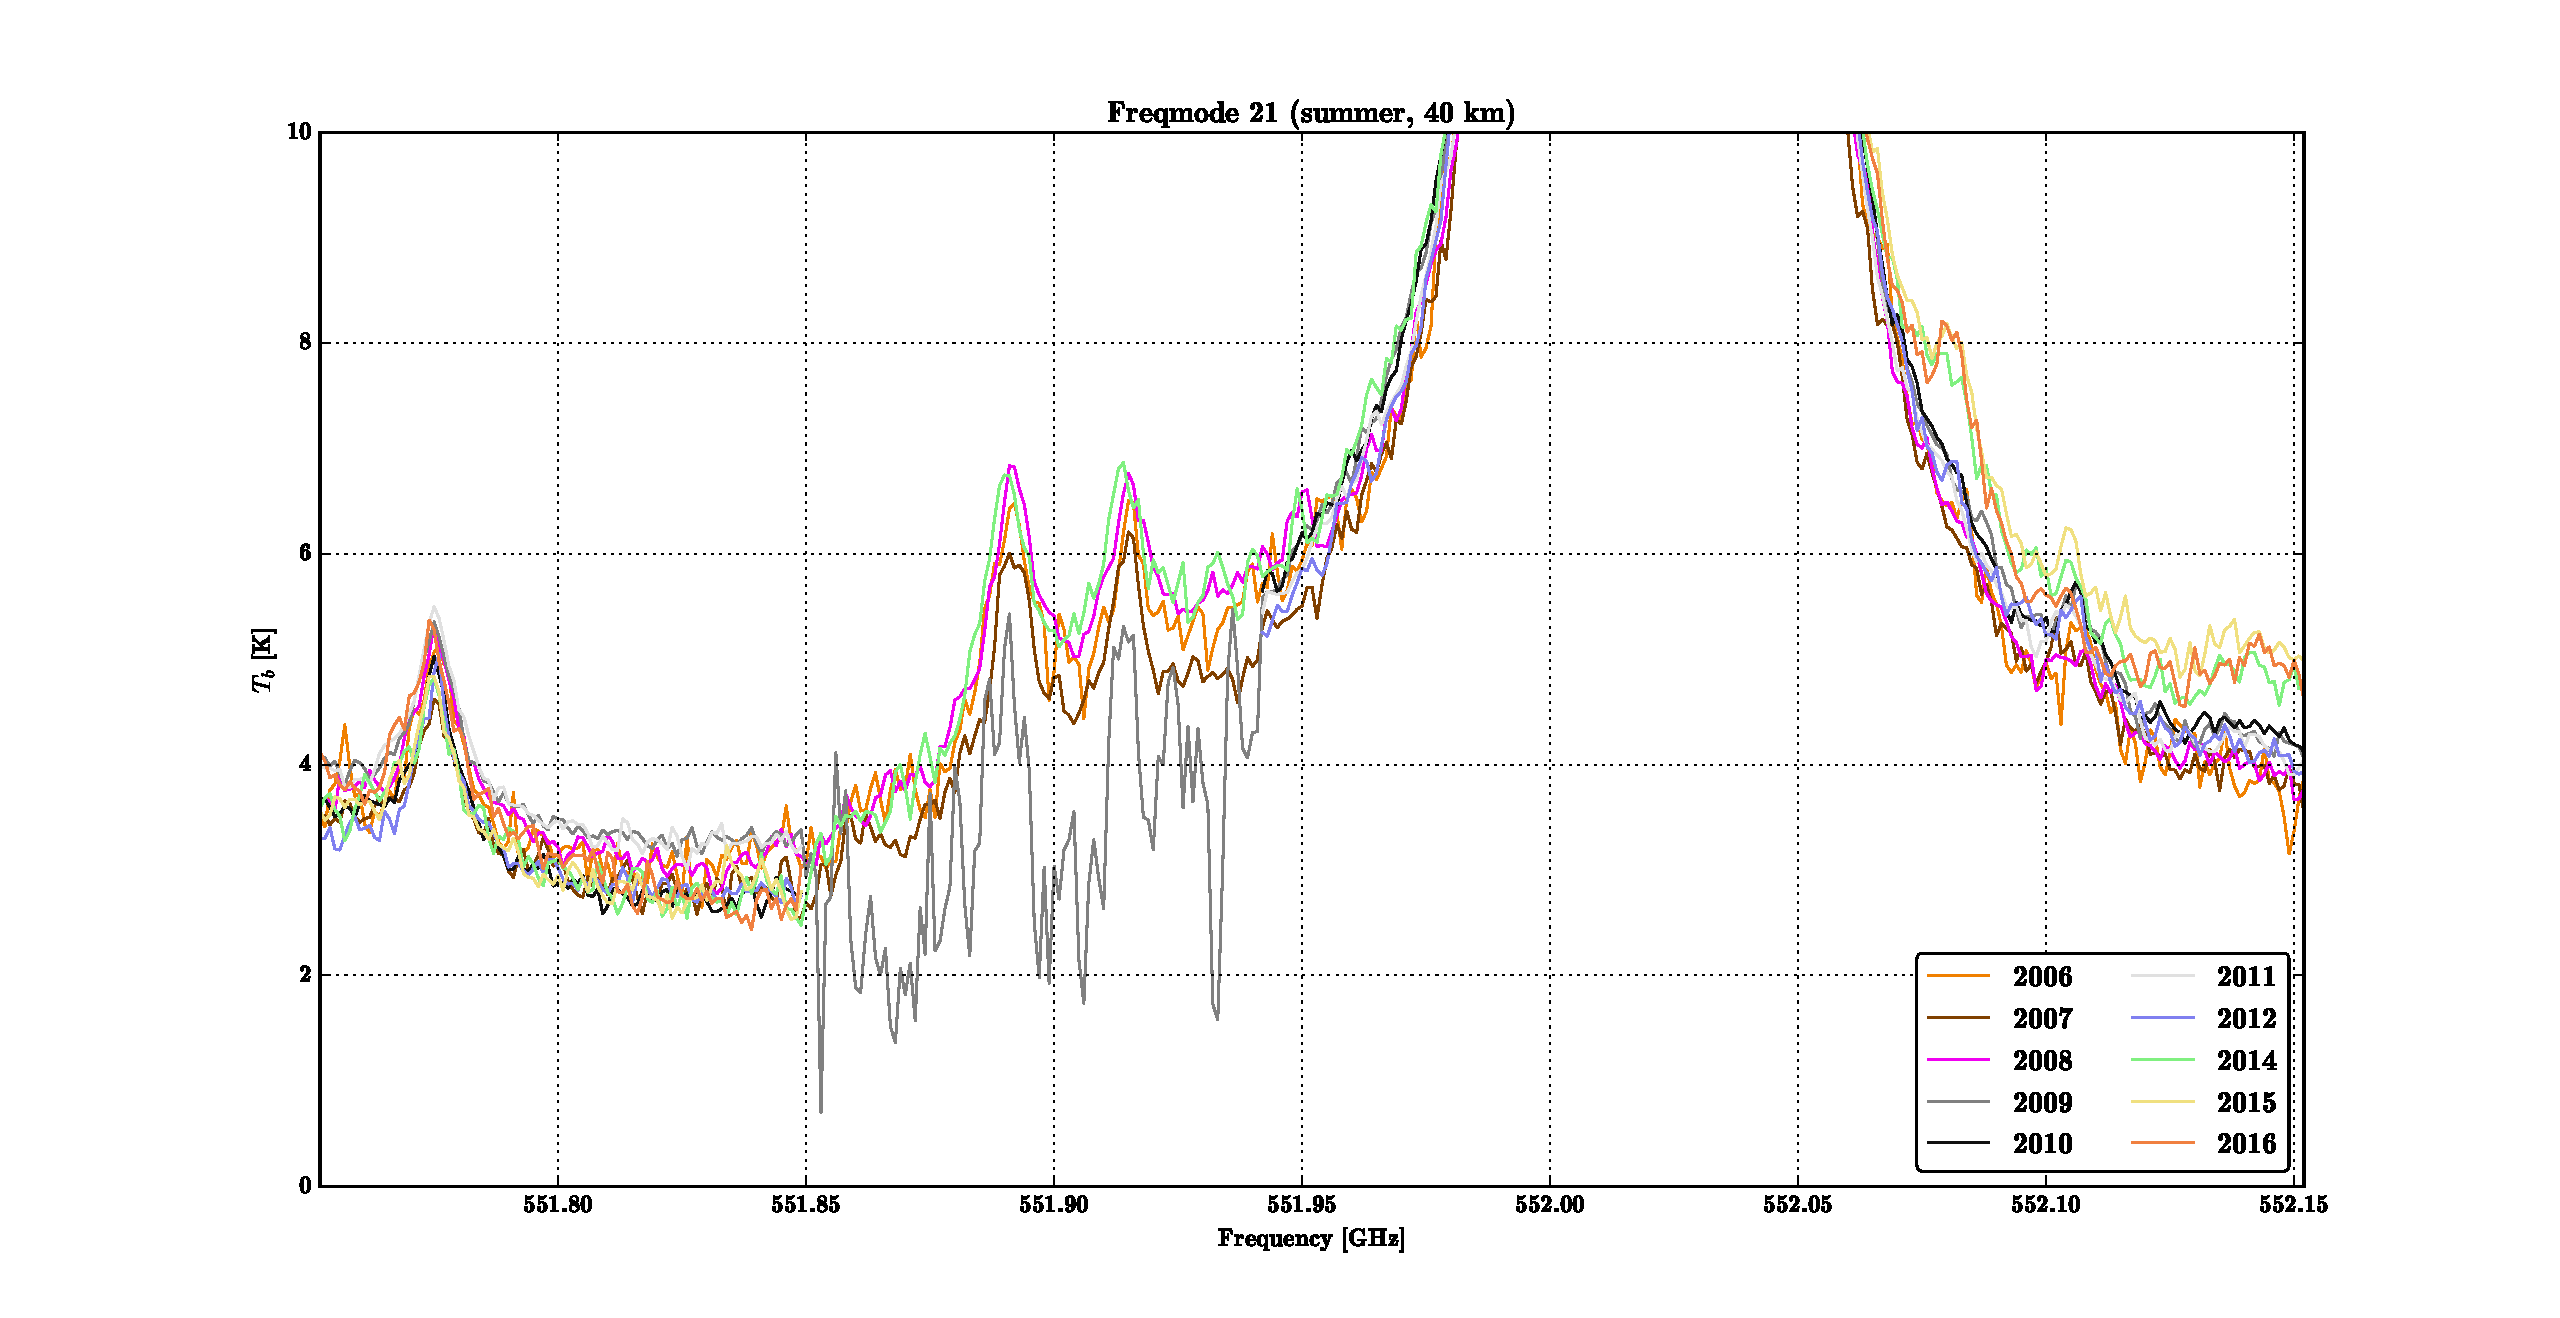
\includegraphics[width=\textwidth]{spectra/fm_21_spectra_summer_right_zoom}
        \caption{summer; 2014--2016 from
            FM~121}\label{fig:spectra:21:summer:closeup}
    \end{subfigure}
    \begin{subfigure}[b]{0.9545\textwidth}
        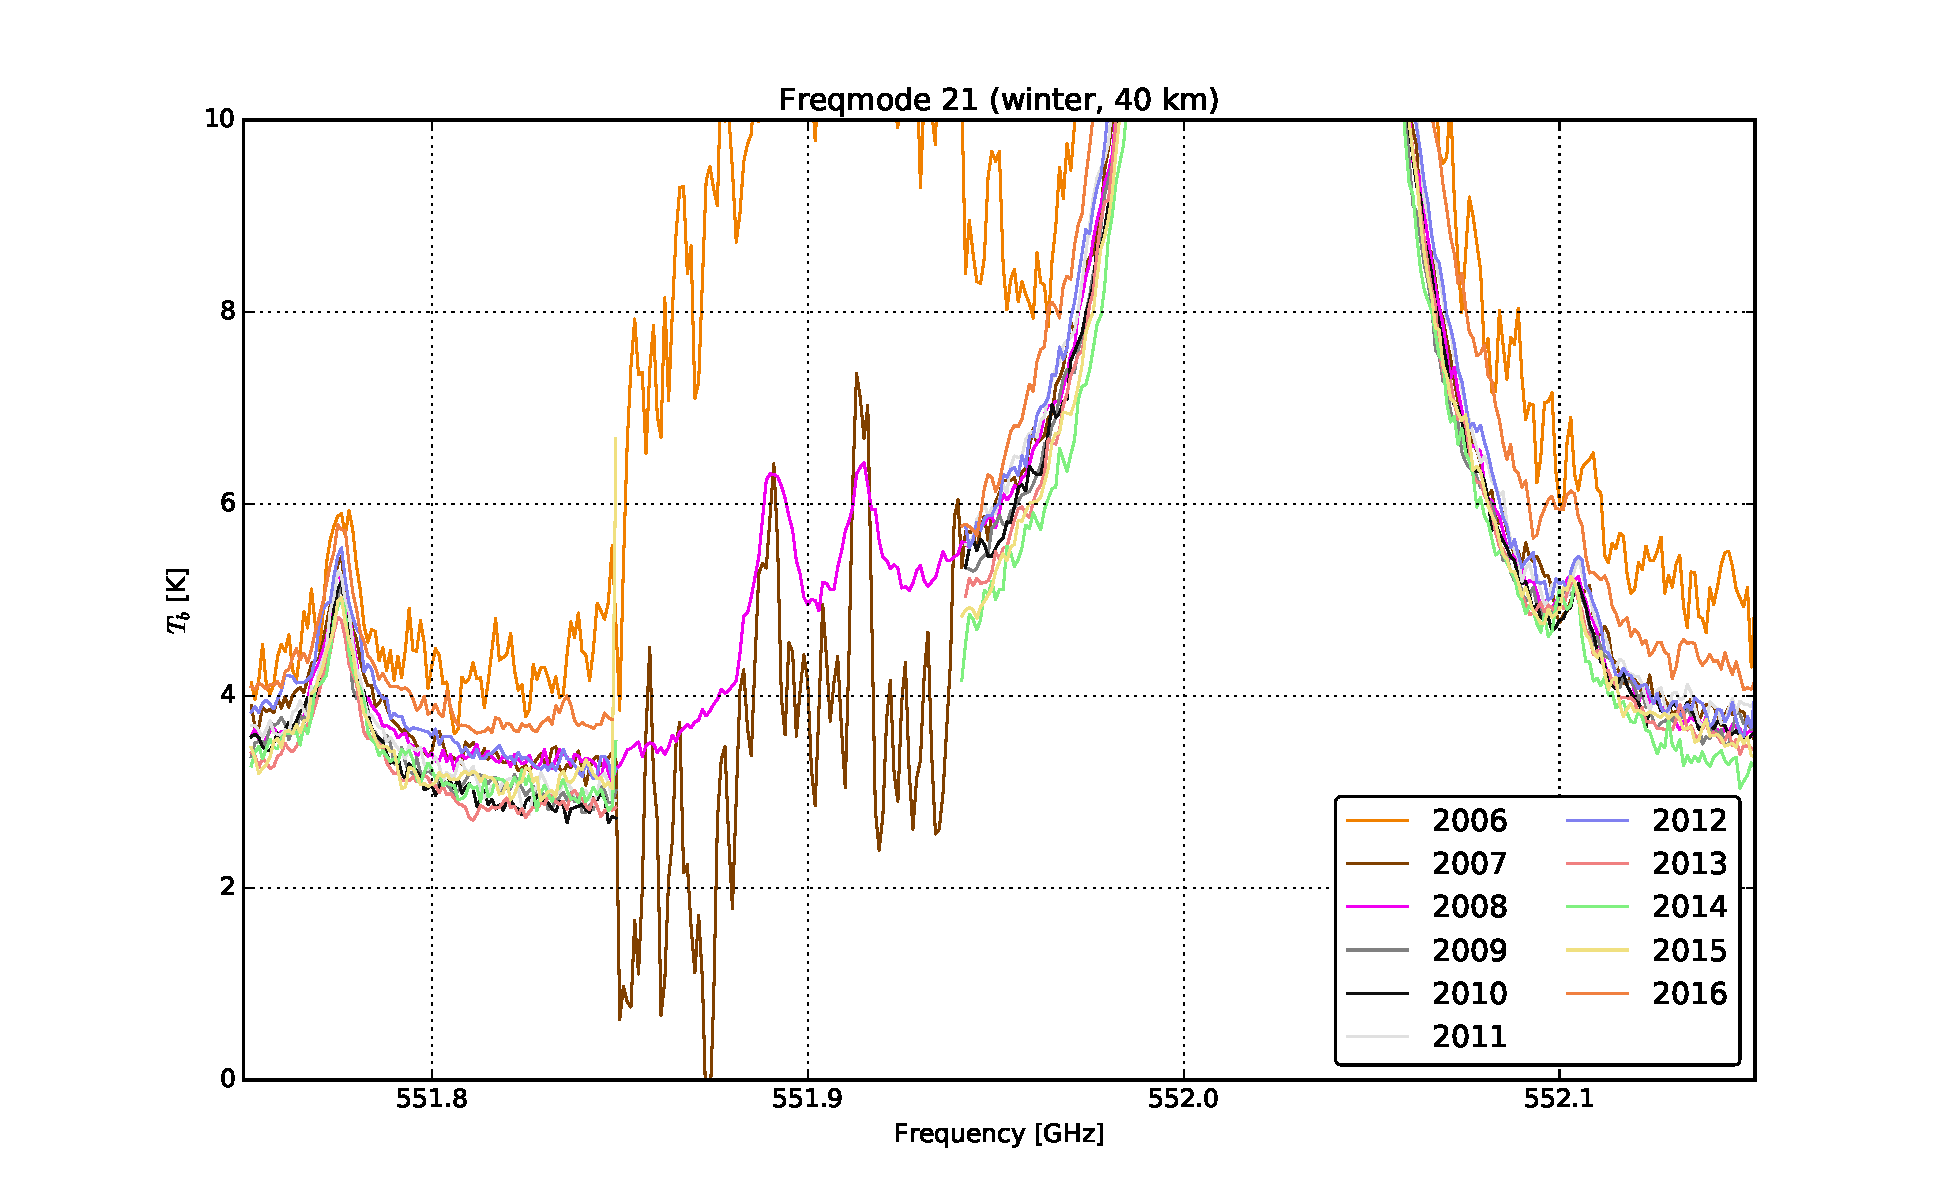
\includegraphics[width=\textwidth]{spectra/fm_21_spectra_winter_right_zoom}
        \caption{winter}\label{fig:spectra:21:winter:closeup}
    \end{subfigure}
    \caption{Close-up of the right side of the annual median spectra for
        FM~21 for altitude interval 35--45~km at equatorial latitudes.  The
        unhealthy sub-bands 2 and 1 are between~$\sim551.75$
        and~$551.95\,\mathrm{GHz}$.
        }\label{fig:spectra:21:closeup}
\end{figure}

\noindent
Yearly median spectra for summer and winter at $\sim40\,\mathrm{km}$ are shown
in Fig.~\ref{fig:spectra:21}.  These, and the close-ups of the right side the
spectrum peak around seen in Fig.~\ref{fig:spectra:21:closeup}, show that the
spectra are fairly consistent over time, with the exception of the winters of
2006 and 2016, when the whole left part of the spectrum appears to have a
positve bias of a few $\mathrm{K}$.

Fig.~\ref{fig:spectra:21:closeup} shows the sideband peaks:  two peaks just
left and right of $551.9\,\mathrm{GHz}$, and one peak just right of
$552.1\,\mathrm{GHz}$.  A closer investigation of the time evolution of these
peaks is presented in Sec.~\ref{FM19:sbl}.


\subsection{Sideband leakage}
\label{FM21:sbl}

\begin{figure}[ht]
    \centering
    \begin{subfigure}[b]{0.9545\textwidth}
        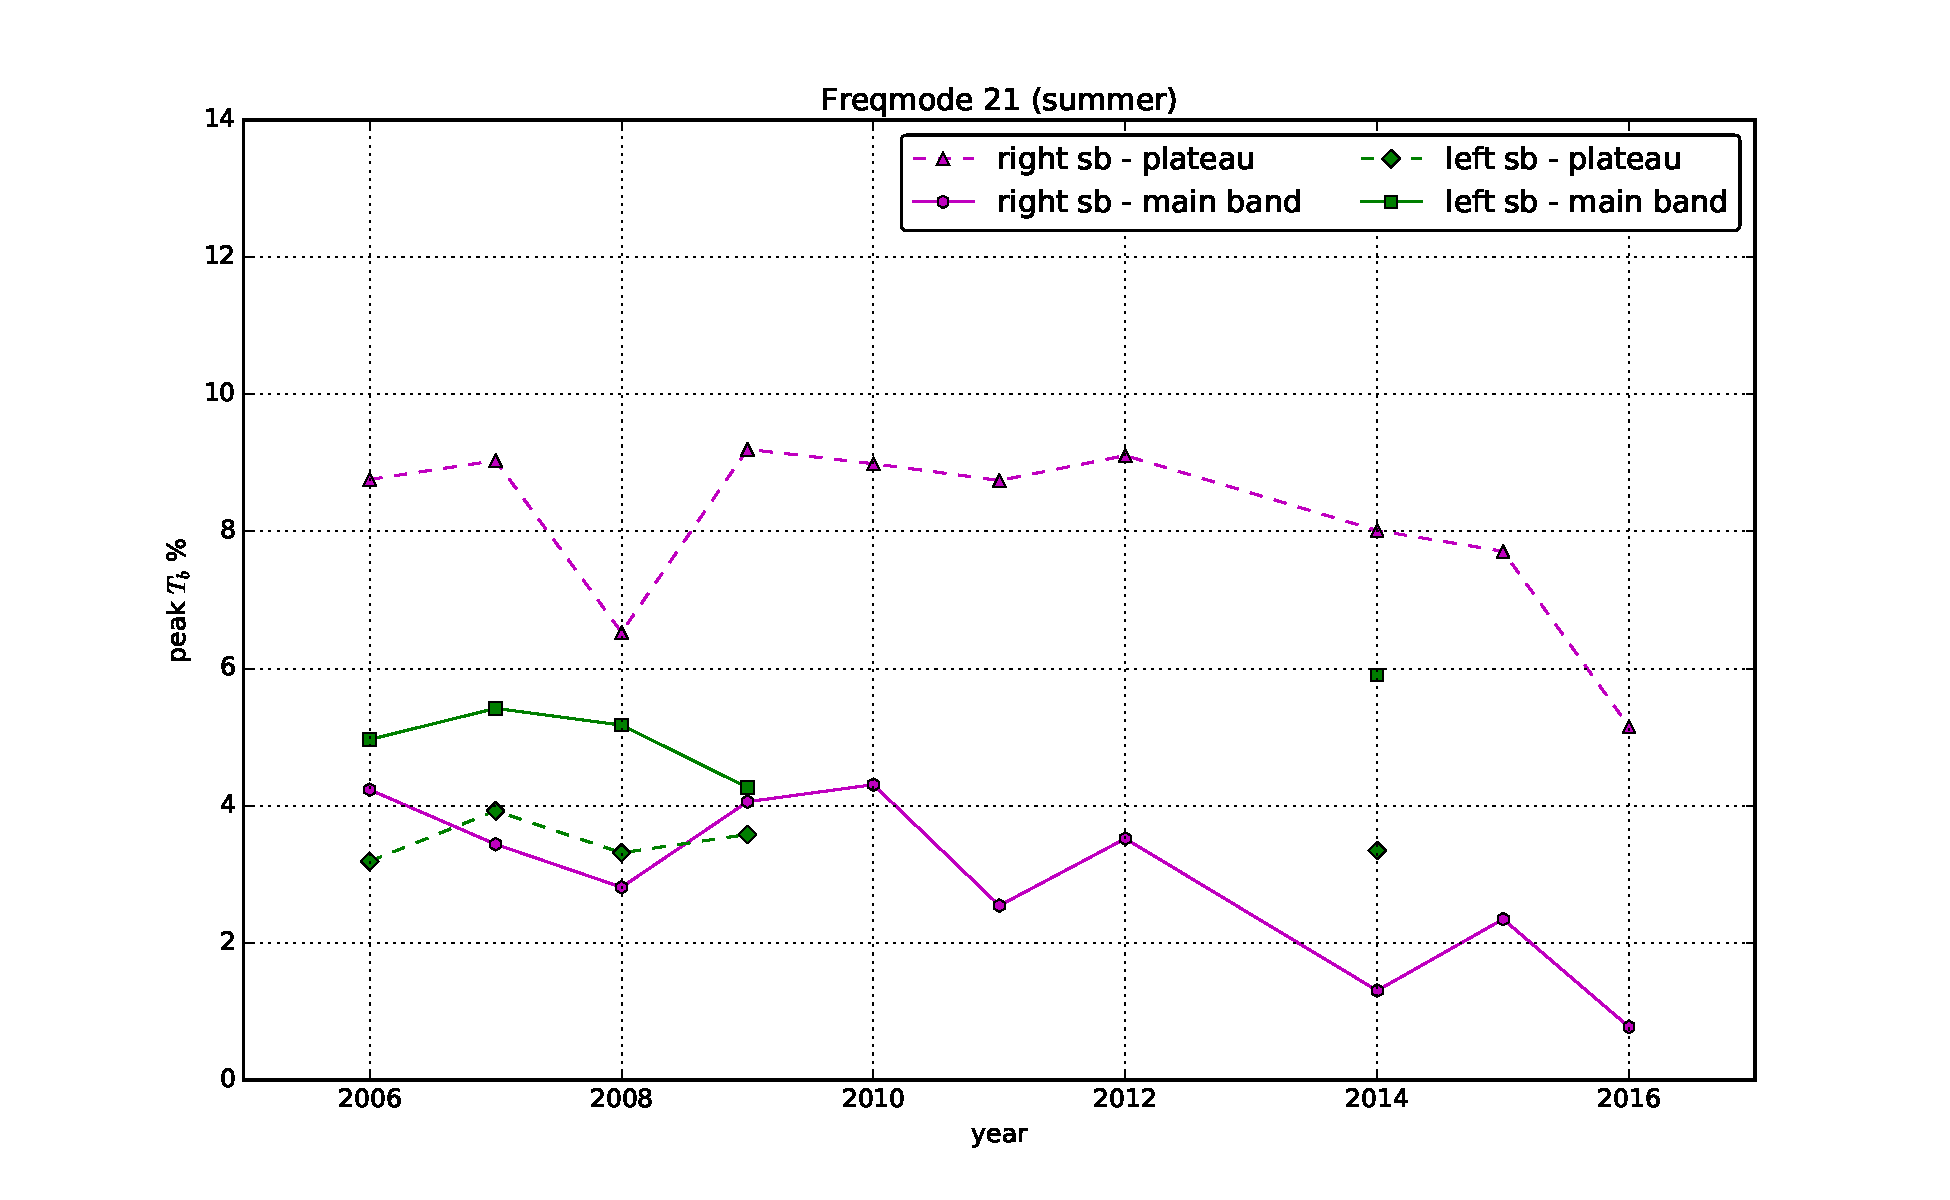
\includegraphics[width=\textwidth]{peaks/fm_21_peaks_summer_40km_sb_adjusted}
        \caption{summer; 2014--2016 from FM~121
            }\label{fig:sbl:21:summer}
    \end{subfigure}
    \begin{subfigure}[b]{0.9545\textwidth}
        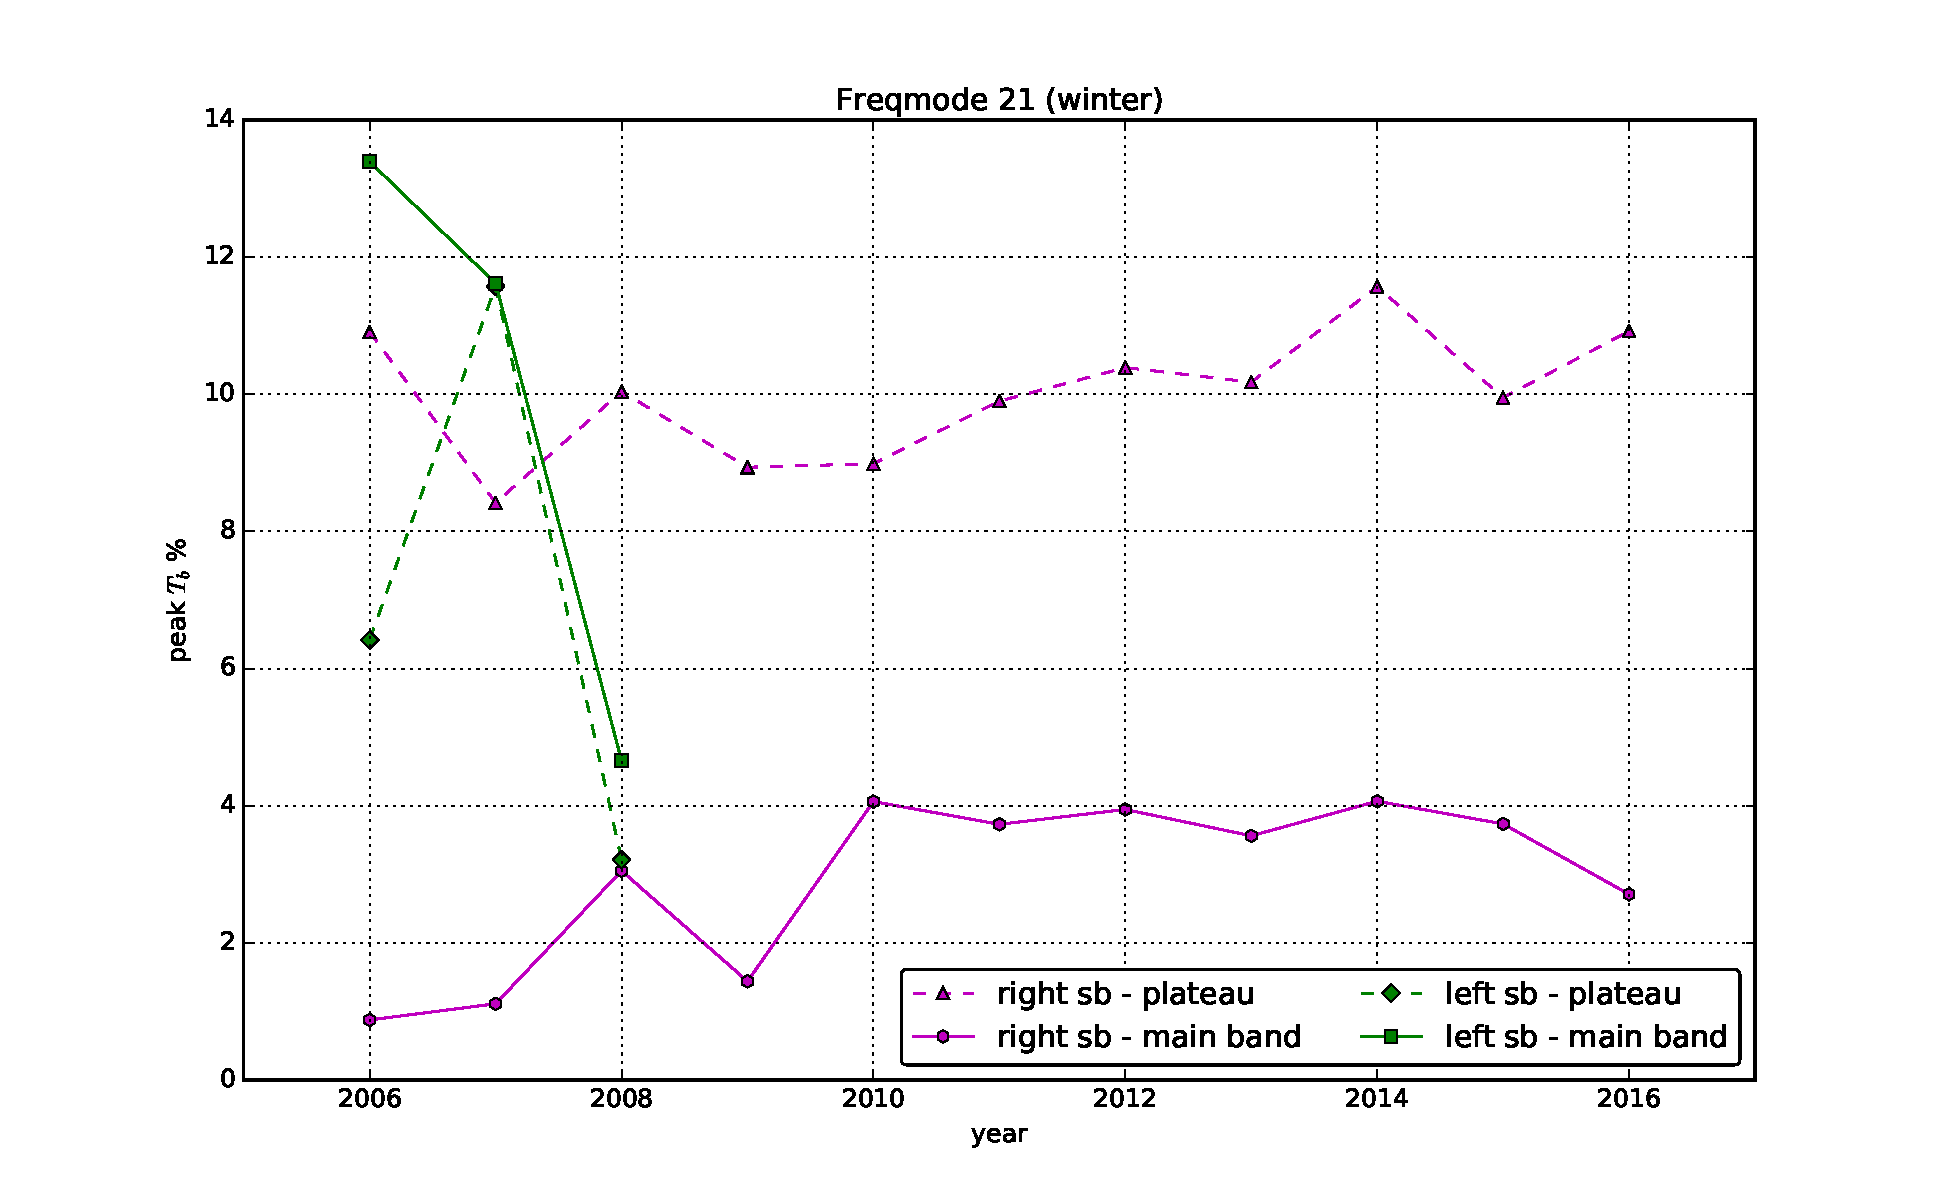
\includegraphics[width=\textwidth]{peaks/fm_21_peaks_winter_40km_sb_adjusted}
        \caption{winter}\label{fig:sbl:21:winter}
    \end{subfigure}
    \caption{Sideband leakage in \% calculated from the data shown in
        Fig.~\ref{fig:spectra:21:closeup}.  Values were calculated by
        subtracting the value of the ``plateau'' on the side of the sideband
        peaks closest to the \chem{H_2^{17}O} peak, or first order
        approximations of the mainband values under the sideband peaks.  The
        results were compared with $34.48\,\mathrm{K}$ (left sideband peak) or
        $14.75\,\mathrm{K}$ (right sideband peak), values deemed
        representative of the actual peak intensities.
        }\label{fig:sbl:21}
\end{figure}

\noindent
The sideband leakage was estimated at $\sim40\,\mathrm{km}$ by taking the
sideband peak intensity from the data shown in
Fig.~\ref{fig:spectra:21:closeup}. The values of the peaks just to the right
of~$551.9$ and~$552.1\,\mathrm{GHz}$ were estimated by and subtracing a the
mainband intensity estimated by two methods:  by taking the value of the
``plateaus'' to the right and left of the respective peaks as the main band
value, and by making first order approximation of the value directly under the
peaks.  The actual value should between these two estimates, but closer to the
latter.

To estimate the leakage, the extracted peak intensities were then
divided by an expected sideband peak intensities from simulations using
ARTS~(\cite{buehler:artst:05}).  $34.38$~and $14.75\,\mathrm{K}$ were chosen as
representative values for the left and right sideband peaks respectively, but
the peak values vary by $\sim0.1$--$0.5\,\mathrm{K}$ from year to year.  The
results are shown in Fig.~\ref{fig:sbl:21}.

As is evident from Fig.~\ref{fig:spectra:21:closeup}, the left sideband peak is
in a bad subband, wherefore the data is too unreliable to draw any conclusions
regarding long term trends. In particular for the winter only the data for 2008
is credible at all, with an estimated sideband leakage of between~4 and~5\%.
For the summer the sideband leakage is also $\sim$5\%, perhaps a little higher
for 2014, where the data is from FM~121.

For the right sideband peak, the leakage appears to have been constant at about
4\% during the (cold) summers for the AC1~backend and at about 2\% for
2014--2016 when the was from from FM~121 which uses the AC2~backend.
During the (warm) winter, when the AC1~backend is always used, the  sideband
leakage appears to have been at a lower level before 2010, wherafter it is more
or less stable at 4\%.


\subsection{Seasonality}
\label{FM21:seasonality}
The peak values of the largest \chem{O_3} line at $\sim45\,\mathrm{km}$ during the
winter are consistently $\sim10\,\mathrm{K}$ higher than during the summer, as
can be seen in Fig.~\ref{fig:spectra:21}.  This could be due to natural
variations in the atmosphere or due to onboard conditions, though as
Fig.~\ref{fig:sbl:21} shows it cannot be attributed to an increased sideband
leakage during the summer when the satellite is colder (see~\ref{sec:Tcal}).
See Sec.~\ref{FM21:sbl} for a more detailed discussion of the seasonality of
the sideband leakage.
